% !TEX root = ../Thesis.tex
\subsection{Validation Results}

This section presents a comprehensive performance evaluation of the RVV64\_Library kernels executed on the Ara vector coprocessor using a cycle-accurate RTL simulation environment. The benchmarking suite targets fundamental operations essential for modern deep learning workloads. Within the scope of this thesis, we focus exclusively on kernels that have been successfully validated using our current infrastructure; more complex operations—such as those involving transcendental functions or highly non-linear reductions—are deferred to future work, as their accurate characterization requires more advanced benchmarking methodologies and architectural insight.

Unless otherwise noted, all reported speedups are relative to an optimized scalar C baseline compiled for the same RISC-V core without vector extensions enabled. The scalar baseline was compiled using Clang/LLVM (from the riscv-llvm toolchain) with the following key flags to ensure high optimization while explicitly preventing any automatic vectorization:

\begin{itemize}
    \item \texttt{-O3} — maximum compiler optimization level for best scalar performance
    \item \texttt{-ffast-math} — enables aggressive floating-point optimizations (reduced precision where allowed)
    \item \texttt{-fno-vectorize} — disables loop auto-vectorization by the compiler
    \item \texttt{-mllvm -scalable-vectorization=off} — turns off the scalable vectorizer pass (prevents generation of RVV code)
    \item \texttt{-mllvm -riscv-v-vector-bits-min=0} — disables assumptions about minimum vector length, avoiding unwanted scalar fallback
    \item \texttt{-march=rv64gcv\_zfh} — base architecture specification (vector parts ignored in scalar baseline)
    \item \texttt{-mabi=lp64d} — consistent 64-bit ABI with double-precision floating-point
\end{itemize}

\subsubsection{Performance Overview}

The benchmarked kernels are categorized into three distinct classes based on their computational and memory access patterns: \textbf{Compute-Bound FMA}, \textbf{Sliding Window \& Filters}, and \textbf{Pointwise \& Elementwise}. Table~\ref{tab:peak_speedups} provides a summary of the peak acceleration achieved in each category.

\begin{table}[H]
\centering
\caption{Peak speedup across all evaluated configurations for each RVV64\_Library kernel.}
\label{tab:peak_speedups}
\vspace{1em}
\begin{tabular}{l l r}
\toprule
\textbf{Category} & \textbf{Kernel} & \textbf{Peak Speedup} \\
\midrule
\textbf{Compute-Bound FMA} & Matrix Multiplication & 70.27$\times$ \\
                           & Dense (Fully Connected) & 4.01$\times$ \\
\midrule
\textbf{Sliding Window \& Filters} & Convolution (IM2COL) & 29.60$\times$ \\
                                   & Max Pooling & 23.48$\times$ \\
\midrule
\textbf{Pointwise \& Elementwise} & Leaky ReLU & 36.02$\times$ \\
                                  & Batch Normalization & 25.01$\times$ \\
                                  & Bias Addition & 21.75$\times$ \\
                                  & ReLU Activation & 20.08$\times$ \\
                                  & Tensor Addition & 19.57$\times$ \\
\bottomrule
\end{tabular}
\end{table}

\subsubsection{Compute-Bound FMA Operations}

These kernels are characterized by high arithmetic intensity, where execution time is primarily limited by the throughput of the Vector Floating-Point Units (VFPU).

\textbf{Matrix Multiplication (MatMul):}
As shown in Table~\ref{tab:matmul_full}, MatMul exhibits the highest scalability in the library. Performance improves dramatically as dimensions increase, allowing the hardware to amortize vector startup costs. Unrolled implementations—which optimize register reuse and reduce scalar branch overhead—consistently outperform standard vector loops, peaking at 70.27$\times$ for a $64 \times 64$ matrix.

\begin{table}[H]
\centering
\caption{Matrix Multiplication (MatMul) — Best Implementation per Size}
\label{tab:matmul_full}
\vspace{1em}
\begin{tabular}{l l r r r}
\toprule
\textbf{Matrix Size} & \textbf{Best Implementation} & \textbf{Scalar Cycles} & \textbf{Best Cycles} & \textbf{Speedup} \\
\midrule
$4 \times 4$   & Vector (M1) Unrolled & 972       & 175     & 5.55$\times$ \\
$16 \times 16$ & Vector (M1) Unrolled & 33,802    & 2,532   & 13.35$\times$ \\
$32 \times 32$ & Vector (M1) Unrolled & 249,114   & 9,873   & 25.23$\times$ \\
$64 \times 64$ & Vector (M2) Unrolled & 4,808,029 & 68,417  & \textbf{70.27$\times$} \\
\bottomrule
\end{tabular}
\end{table}

\textbf{Dense (Fully Connected) Layer:}
The Dense layer achieves lower speedups compared to MatMul due to its matrix-vector access pattern, which significantly increases pressure on the memory subsystem and lowers arithmetic intensity. As a result, the kernel becomes memory-bound, and speedup is limited by the available memory bandwidth rather than by the peak throughput of the vector floating-point units.

\begin{table}[H]
\centering
\caption{Dense (Fully Connected) Layer — Best Implementation per Size}
\label{tab:dense_full}
\vspace{1em}
\begin{tabular}{l l l r r r}
\toprule
\textbf{Input Size} & \textbf{Output Size} & \textbf{Best Implementation} & \textbf{Scalar Cycles} & \textbf{Best Cycles} & \textbf{Speedup} \\
\midrule
64  & 64  & Vector (M8) & 37,076   & 10,225  & 3.63$\times$ \\
128 & 128 & Vector (M8) & 146,576  & 38,150  & 3.84$\times$ \\
256 & 256 & Vector (M8) & 589,635  & 147,133 & \textbf{4.01$\times$} \\
\bottomrule
\end{tabular}
\end{table}
	

\subsubsection{Sliding Window \& Filters}

\textbf{Convolution (Conv):}
As summarized in Table~\ref{tab:conv_full}, IM2COL combined with GEMM significantly outperforms direct convolution for large inputs and filter sets. For very small inputs such as $[1,4,4]$ with a single filter, the scalar baseline remains competitive once vector setup overhead is taken into account, but at $[1,32,32]$ with 32 filters IM2COL + GEMM becomes essential, achieving a speedup of \textbf{29.60$\times$}.

\begin{table}[H]
\centering
\caption{Convolution (Conv) — Best Implementation per Configuration}
\label{tab:conv_full}
\vspace{1em}
\begin{tabular}{l l l l r r r}
\toprule
\textbf{Input Shape} & \textbf{Filters} & \textbf{Kernel} & \textbf{Best Implementation} & \textbf{Scalar Cycles} & \textbf{Best Cycles} & \textbf{Speedup} \\
\midrule
$[1,4,4]$   & 1  & $3\times3$ & Scalar (baseline)       & 1,875        & 1,875        & 1.00$\times$ \\
$[1,8,8]$   & 2  & $3\times3$ & IM2COL + GEMM (M8)      & 20,625       & 5,629        & 3.67$\times$ \\
$[1,32,32]$ & 6  & $5\times5$ & IM2COL + GEMM (M8)      & 2,969,298    & 134,698      & 22.04$\times$ \\
$[1,32,32]$ & 32 & $5\times5$ & IM2COL + GEMM (M8)      & 15,826,364   & 534,683      & \textbf{29.60$\times$} \\
\bottomrule
\end{tabular}
\end{table}

\textbf{Max Pooling:}
As shown in Table~\ref{tab:maxpool_full}, max pooling performance is highly sensitive to both input size and stride. Moving from $[1,16,16]$ to $[1,64,64]$ and using stride 1 increases the number of output elements and improves vector utilization, resulting in the peak speedup of \textbf{23.48$\times$}. Conversely, larger strides reduce the number of outputs and lead to lower speedups despite similar computation per window.

\begin{table}[H]
\centering
\caption{MaxPool — Best Vector Implementation (M8) per Configuration}
\label{tab:maxpool_full}
\vspace{1em}
\begin{tabular}{l l r r r}
\toprule
\textbf{Input Shape} & \textbf{Pool / Stride} & \textbf{Scalar Cycles} & \textbf{Vector Cycles (M8)} & \textbf{Speedup} \\
\midrule
$[1,16,16]$ & $2\times2$ / 1 & 17,721  & 2,286  & 7.75$\times$ \\
$[1,16,16]$ & $2\times2$ / 2 & 5,895   & 1,836  & 3.21$\times$ \\
$[1,64,64]$ & $2\times2$ / 2 & 82,213  & 12,254 & 6.71$\times$ \\
$[1,64,64]$ & $2\times2$ / 1 & 295,391 & 12,578 & \textbf{23.48$\times$} \\
\bottomrule
\end{tabular}
\end{table}

\subsubsection{Pointwise \& Elementwise Operations}

\textbf{Activation Functions (ReLU / Leaky ReLU):}

\begin{table}[H]
\centering
\caption{ReLU and Leaky ReLU — Best Vector Implementation (M8)}
\label{tab:act_full}
\vspace{1em}
\begin{tabular}{l l r r r}
\toprule
\textbf{Kernel} & \textbf{Input Size} & \textbf{Scalar Cycles} & \textbf{Vector Cycles (M8)} & \textbf{Speedup} \\
\midrule
ReLU       & $32 \times 32$   & 12,023     & 649      & 18.53$\times$ \\
ReLU       & $128 \times 128$ & 190,583    & 9,529    & 20.00$\times$ \\
ReLU       & $256 \times 256$ & 761,975    & 37,945   & 20.08$\times$ \\
\midrule
Leaky ReLU & $32 \times 32$   & 19,388     & 629      & 30.82$\times$ \\
Leaky ReLU & $128 \times 128$ & 307,938    & 8,609    & 35.77$\times$ \\
Leaky ReLU & $256 \times 256$ & 1,230,050  & 34,145   & \textbf{36.02$\times$} \\
\bottomrule
\end{tabular}
\end{table}

ReLU and Leaky ReLU both benefit strongly from vectorization, as shown in Table~\ref{tab:act_full}. For ReLU, the speedup quickly saturates around $20\times$ as the input size grows, indicating that performance becomes primarily limited by memory bandwidth rather than computation. Leaky ReLU achieves even higher speedups, up to \textbf{36.02$\times$} for a $256 \times 256$ input, because the scalar baseline relies on conditional branches while the vectorized version uses mask-based or branch-free arithmetic, reducing branch overhead and improving utilization of the vector units. \\

\textbf{Batch Normalization:}

\begin{table}[H]
\centering
\caption{Batch Normalization — Best Vector Implementation (M8)}
\label{tab:batch_full}
\vspace{1em}
\begin{tabular}{l r r r}
\toprule
\textbf{Input Shape} & \textbf{Scalar Cycles} & \textbf{Vector Cycles (M8)} & \textbf{Speedup} \\
\midrule
$[1,6,14]$   & 1,714   & 250    & 6.86$\times$ \\
$[1,64,8]$   & 8,876   & 509    & 17.44$\times$ \\
$[1,128,32]$ & 68,914  & 2,755  & \textbf{25.01$\times$} \\
\bottomrule
\end{tabular}
\end{table}

Table~\ref{tab:batch_full} shows that batch normalization also gains substantial speedups from vectorization, increasing from $6.86\times$ for the smallest shape $[1,6,14]$ to \textbf{25.01$\times$} for $[1,128,32]$. Larger input shapes expose more parallel work per invocation, allowing the M8 configuration to keep the vector pipelines busy while amortizing setup overhead. The reported speedups are measured relative to a scalar baseline implementation that applies the same batch normalization equations without vector extensions. \\

\textbf{Additive Kernels (Bias Add / Tensor Add):}

\begin{table}[H]
\centering
\caption{Additive Kernels — Best Implementation per Size}
\label{tab:add_full}
\vspace{1em}
\begin{tabular}{l l l r r r}
\toprule
\textbf{Kernel} & \textbf{Size / Shape} & \textbf{Best Implementation} & \textbf{Scalar Cycles} & \textbf{Best Cycles} & \textbf{Speedup} \\
\midrule
Bias Add   & $1 \times 8 \times 32 \times 32$ & Vector (M8) & 103,759   & 4,931    & 21.04$\times$ \\
Bias Add   & $1 \times 8 \times 64 \times 64$ & Vector (M8) & 414,096   & 19,043   & \textbf{21.75$\times$} \\
\midrule
Tensor Add & 1,024 Elements                 & Vector (M8) & 15,938    & 889      & 17.93$\times$ \\
Tensor Add & 16,384 Elements                & Vector (M8) & 265,236   & 13,609   & 19.49$\times$ \\
Tensor Add & 65,536 Elements                & Vector (M8) & 1,062,966 & 54,313   & \textbf{19.57$\times$} \\
\bottomrule
\end{tabular}
\end{table}

As summarized in Table~\ref{tab:add_full}, additive kernels achieve consistent and high speedups across all evaluated sizes. Bias addition reaches up to \textbf{21.75$\times$} for the $1 \times 8 \times 64 \times 64$ tensor, where contiguous channel-wise accesses map efficiently onto M8 vectors. Tensor addition shows increasing speedup with problem size, from $17.93\times$ at 1{,}024 elements to \textbf{19.57$\times$} at 65{,}536 elements, after which performance is effectively capped by memory bandwidth rather than arithmetic throughput.

\subsubsection{Results Discussion}

The performance evaluation of the Ara vector coprocessor demonstrates that vectorization can deliver substantial acceleration across a variety of computational kernels, spanning \textbf{compute-bound FMA operations}, \textbf{sliding window convolutions}, and \textbf{pointwise elementwise operations}. In this section, we interpret the measured results, highlight comparative trends, and discuss the influence of vector length (LMUL), tiling strategies, and arithmetic intensity on the observed speedups.

\paragraph{Compute-Bound Operations (MatMul \& Dense Layers)} 

Matrix multiplication (MatMul) benefits the most from Ara's vector architecture. Table~\ref{tab:matmul_full} shows that unrolled vector implementations achieve speedups up to \textbf{70.27$\times$} for a $64 \times 64$ matrix. This dramatic improvement arises from several factors: 

\begin{itemize}
	\item \textbf{Instruction-Level Parallelism:} By unrolling loops and reusing registers, the scalar overhead is minimized and vector pipelines remain fully occupied.
	\item \textbf{Vector Startup Amortization:} For small matrices ($4\times4$), vector setup overhead dominates, yielding only moderate speedups ($\sim5.5\times$). As matrix dimensions increase, this overhead is amortized across more multiply-accumulate (MAC) operations, revealing the true hardware potential.
	\item \textbf{LMUL Scaling:} Increasing LMUL beyond M1 provides marginal improvement for small sizes but becomes critical for large matrices, enabling longer vector chains and better register utilization.
\end{itemize}

Dense layers, which essentially perform matrix-vector multiplications, show lower speedups (max $\sim4\times$ for $256 \times 256$). The reduced gains are largely due to the memory-bound nature of matrix-vector operations: memory bandwidth limits the effective utilization of the vector functional units. Comparing MatMul and Dense highlights the importance of operational intensity: compute-bound operations benefit far more from Ara's vector units than memory-bound vector operations.

\begin{figure}[H]
\centering
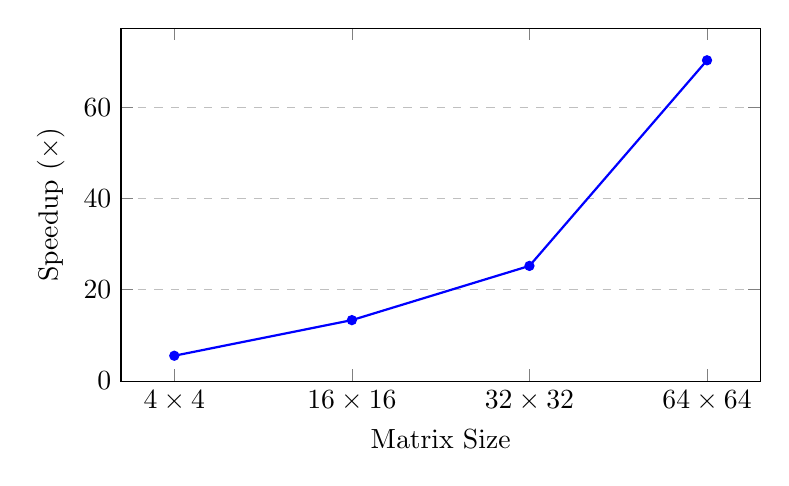
\begin{tikzpicture}
	\begin{axis}[
		width=0.8\textwidth,
		height=0.5\textwidth,
		xlabel={Matrix Size},
		ylabel={Speedup ($\times$)},
		xtick={1,2,3,4},
		xticklabels={$4\times4$, $16\times16$, $32\times32$, $64\times64$},
		ymin=0,
		ymajorgrids=true,
		grid style=dashed,
		mark options={scale=1.2}
	]
	\addplot[
		blue,
		thick,
		mark=*,
		mark size=1.2pt,
	]
	coordinates {
		(1,5.55) (2,13.35) (3,25.23) (4,70.27)
	};
	\end{axis}
	\end{tikzpicture}
	\caption{Speedup of MatMul across matrix sizes}
	\label{fig:matmul_speedup}
\end{figure}

\paragraph{Sliding Window Operations (Convolution \& Max Pooling)}

Sliding window operations, such as convolution and max pooling, display highly input-dependent performance characteristics. Convolution kernels benefit significantly from \textbf{IM2COL transformations combined with GEMM} for large input shapes and filter counts. For instance, while direct convolution is competitive for very small inputs like $[1,4,4]$, it becomes extremely inefficient at $[1,32,32]$ with 32 filters. IM2COL + GEMM achieves a speedup of \textbf{29.60$\times$}, demonstrating that reorganizing data into a matrix format allows the vector units to be fully utilized, similar to dense matrix multiplication.

Max pooling shows a different trend: its performance is sensitive to both stride and input size. Larger inputs ($[1,64,64]$) with stride 1 achieve the highest speedup ($23.48\times$) using vectorization, whereas small inputs or larger strides exhibit lower speedups due to a smaller number of output elements and vector underutilization. Unlike convolution, max pooling is less amenable to memory transformations such as IM2COL; the primary improvement comes from wider vectorization (M8) reducing loop overhead and scalar instructions.

\paragraph{Pointwise and Elementwise Operations (Activation \& Additive Kernels)}

Pointwise kernels, including ReLU, Leaky ReLU, batch normalization, and additive operations, exhibit strong benefits from wider vectors. Increasing LMUL to M8 often saturates memory bandwidth, reducing vector instruction count and yielding speedups up to \textbf{36.02$\times$} for Leaky ReLU ($256 \times 256$) and \textbf{21.75$\times$} for bias addition ($1\times8\times64\times64$). 

Key observations include:

\begin{itemize}
    \item \textbf{Vector Length Effect:} In our experiments (not all configurations are tabulated), moving from M1 to M8 consistently decreases cycles, with diminishing returns for very small sizes.
    \item \textbf{Memory-Bound Saturation:} For large arrays (e.g., Tensor Add with 65,536 elements), speedup is capped at $\sim20\times$, indicating memory bandwidth limitations.
    \item \textbf{Activation Functions:} Leaky ReLU benefits more than ReLU because the scalar baseline relies on conditional branching, whereas the vectorized implementation uses mask-based or branch-free arithmetic, avoiding branch penalties.
    \item \textbf{Batch Normalization:} Speedups scale with both vector width and input shape, reaching \textbf{25.01$\times$} for $[1,128,32]$.
\end{itemize}

\paragraph{Overall Analysis}

\begin{enumerate}
    \item \textbf{Small vs Large Problem Sizes:} Very small problem sizes often see marginal speedups or even slowdowns. This is due to vector setup and loop overhead dominating execution time. For example, MatMul $4 \times 4$ only achieves $5.55\times$ speedup.
    \item \textbf{Compute-Bound vs Memory-Bound:} Compute-bound operations (MatMul, Conv-IM2COL) achieve the largest speedups, whereas memory-bound operations (Dense, Additive Kernels, Pointwise) are limited by the bandwidth of the memory subsystem, saturating at approximately $20\times$ for largest vectors.
    \item \textbf{Vectorization Strategy:} Unrolling, tiling, and maximizing LMUL are essential techniques to approach peak Ara performance. Tiled versions sometimes reduce speedup for small inputs due to overhead but help with cache locality in medium-to-large inputs.
    \item \textbf{Implementation Selection:} The tables highlight that the best implementation depends on size and kernel type. For instance, IM2COL + GEMM is essential for large convolutions, M8 is ideal for additive and activation kernels, and unrolled vector loops excel for MatMul.
\end{enumerate}

